% Template for PLoS
% Version 2.0 July 2014
%
% To compile to pdf, run:
% latex plos.template
% bibtex plos.template
% latex plos.template
% latex plos.template
% dvipdf plos.template
%!TEX encoding = UTF-8 Unicode
% % % % % % % % % % % % % % % % % % % % % %
%
% -- IMPORTANT NOTE
%
% Be advised that this is merely a template 
% designed to facilitate accurate translation of manuscript content 
% into our production files. 
%
% This template contains extensive comments intended 
% to minimize problems and delays during our production 
% process. Please follow the template 
% whenever possible.
% % % % % % % % % % % % % % % % % % % % % % % 
%
% Once your paper is accepted for publication and enters production, 
% PLEASE REMOVE ALL TRACKED CHANGES in this file and leave only
% the final text of your manuscript.
%
% DO NOT ADD EXTRA PACKAGES TO THIS TEMPLATE unless absolutely necessary.
% Packages included in this template are intentionally
% limited and basic in order to reduce the possibility
% of issues during our production process.
%
% % % % % % % % % % % % % % % % % % % % % % %
%
% -- FIGURES AND TABLES
%
% DO NOT INCLUDE GRAPHICS IN YOUR MANUSCRIPT
% - Figures should be uploaded separately from your manuscript file. 
% - Figures generated using LaTeX should be extracted and removed from the PDF before submission. 
% - Figures containing multiple panels/subfigures must be combined into one image file before submission.
% See http://www.plosone.org/static/figureGuidelines for PLOS figure guidelines.
%
% Tables should be cell-based and may not contain:
% - tabs/spacing/line breaks within cells to alter layout
% - vertically-merged cells (no tabular environments within tabular environments, do not use \multirow)
% - colors, shading, or graphic objects
% See http://www.plosone.org/static/figureGuidelines#tables for table guidelines.
%
% For sideways tables, use the {rotating} package and use \begin{sidewaystable} instead of \begin{table} in the appropriate section. PLOS guidelines do not accomodate sideways figures.
%
% % % % % % % % % % % % % % % % % % % % % % % %
%
% -- EQUATIONS, MATH SYMBOLS, SUBSCRIPTS, AND SUPERSCRIPTS
%
% IMPORTANT
% Below are a few tips to help format your equations and other special characters according to our specifications. For more tips to help reduce the possibility of formatting errors during conversion, please see our LaTeX guidelines at http://www.plosone.org/static/latexGuidelines
%
% Please be sure to include all portions of an equation in the math environment, and for any superscripts or subscripts also include the base number/text. For example, use $mathrm{mm}^2$ instead of mm$^2$ (do not use the\textsuperscript command).
%
% DO NOT USE the \rm command to render mathmode characters in roman font, instead use $\mathrm{}$
% For bolding characters in mathmode, please use $\mathbf{}$ 
%
% Please add line breaks to long equations when possible in order to fit our 2-column layout. 
%
% For inline equations, please do not include punctuation within the math environment unless this is part of the equation.
%!TEX encoding = UTF-8 Unicode
% For spaces within the math environment please use the \; or \: commands, even within \text{} (do not use smaller spacing as this does not convert well).
%
%!TEX encoding = UTF-8 Unicode
% % % % % % % % % % % % % % % % % % % % % % % %



\documentclass[10pt]{article}
\usepackage{colortbl}

% amsmath package, useful for mathematical formulas
\usepackage{amsmath}
% amssymb package, useful for mathematical symbols
\usepackage{amssymb}

% cite package, to clean up citations in the main text. Do not remove.
\usepackage{cite}
 
\usepackage{hyperref}

% line numbers
\usepackage{lineno}
 
 % ligatures disabled
\usepackage{microtype}
\usepackage{graphicx} 
 
\DisableLigatures[f]{encoding = *, family = * }

% rotating package for sideways tables
%\usepackage{rotating}

% If you wish to include algorithms, please use one of the packages below. Also, please see the algorithm section of our LaTeX guidelines (http://www.plosone.org/static/latexGuidelines) for important information about required formatting.
%\usepackage{algorithmic}
%\usepackage{algorithmicx}

% Use doublespacing - comment out for single spacing
%\usepackage{setspace} 
%\doublespacing


% Text layout
\topmargin 0.0cm
\oddsidemargin 0.5cm
\evensidemargin 0.5cm
\textwidth 16cm 
\textheight 21cm

% Bold the 'Figure #' in the caption and separate it with a period
% Captions will be left justified
\usepackage[labelfont=bf,labelsep=period,justification=raggedright]{caption}
 

 
 % Remove brackets from numbering in List of References
\makeatletter
\renewcommand{\@biblabel}[1]{\quad#1.}
\makeatother


% Leave date blank
\date{}

\pagestyle{myheadings}

%% Include all macros below. Please limit the use of macros.

%% END MACROS SECTION

 
\begin{document}


% Title must be 150 characters or less
\begin{flushleft}
{\Large
\textbf{Evaluating Metagenome Assembly on a Complex Community}
}
% Insert Author names, affiliations and corresponding author email.
\\
 
Sherine Awad $^{1}$, 
Titus Brown $^{1,\ast}$ 

\bf{1} Population Health and Reproduction
University of California, Davis, Davis, CA, USA 
 
 
$\ast$ E-mail:  ctbrown@ucdavis.edu 
\end{flushleft}

% Please keep the abstract between 250 and 300 words
% Please keep the abstract between 250 and 300 words
\section*{Abstract}
NEEDS ENHANCEMENTS

Motivation: With the emergence of de novo assembly, several work have been to done to assemble metagenomic data from de novo. Several assemblers exist that are based on different assembly techniques. However, we still lack  a study that analyze different assemblers behavior on metagenomic data . 


Problem statement: In this paper, we performed analytical study for metagnome assembly using different assemblers and different preprocessing treatments. The aim of the analysis is studying how well metagenome assembly works, and which assembly works best. In addition, the study analyzes the resource requirements of the assembly. 


Approach: We used a mock community dataset for the analysis, and used its reference genome for benchmark evaluation. We quality filtered the reads, then we applied 2 other preprocessing steps: digital normalization and partitioning. We used 4 different assembler: Velvet, IDBA-UD, SPAdes, and megahit to assemble the reads using each treatment. We used Quast to analyze assemblies accuracy. 


Results: Results show that assembly works well. Velvet is the worst assembler in terms of accuracy and recourses utilizations. The results also showed that assembly counts to most of the reads. 
 
 
Conclusions: Except for Velvet, assemblers works well. Further analysis is required to study which assembler is better used with each specific dataset. This step is left for our future work, 
% Please keep the Author Summary between 150 and 200 words
% Use first person. PLOS ONE authors please skip this step. 
% Author Summary not valid for PLOS ONE submissions.   
\section*{Author Summary}

WHAT SHOULD BE WRITTEN HERE


\section*{Introduction}

 
Metagenome is the sequencing of DNA in an environmental sample. While whole genome sequencing (WGS) usually targets one genome, metagenome targets several ones which introduces complexity to metagenome analyis due to genomic diversity and variable abundance within populations.  Metagenomic assembly  means the assembly of multiple genomes from mixed sequences of reads of multiple species in a microbial community.  
Most approaches for analyzing metagenomic data rely on mapping to reference genomes. However, not all microbial diversity of many environments are covered by reference databases. Hence, the need for de novo assembly of complex metagenomic data rises.  
Several assemblers exist that can be used for de novo assembly. In order to decide which assembly works best, we need to evaluate metagenome assembly generated by each assembler.  In this paper, we provide, an evaluation for metegnome assembly generated by several assemblers and using different preprocessing treatments. We use a reference genome as a benchmark for the evaluation.  The evaluation is based on assembly accuracy, and time and memory requirements. This evaluation shed light on doability of metagenome assembly and the minimum requirements needed for the assembly. In addition, knowing how each assembler works, helps deciding which assembler to use prior to assembly. However, the later point is left for our future work. 
 
The comparative study in this paper is based on four different assemblers; Velvet \cite{velvet}, SPAdes \cite {spades}, IDBA-UD \cite{idba}, and Megahit \cite{megahit}.  


Velvet \cite{velvet} is a group de Bruin graph-based sequence assembly methods for very short reads that can both remove errors. It also uses read pair information to resolve a large number of repeats.  The error correction algorithm merges the sequences that belongs together. Then the repeat solver algorithm separates parts that share overlaps. 


Spades \cite{spades} is an assembler for both single-cell and standard (multicell) assembly. SPAdes generates single-cell assemblies and provides information about genomes of uncultivatable bacteria that vastly exceeds what may be obtained via traditional metagenomics studies. 

IDBA-UD \cite{idba} is a de Bruijn graph approach for assembling reads from single cell sequencing or metagenomic sequencing technologies with uneven sequencing depths. IDBA-UD uses multiple depth-relative thresholds to remove erroneous k-mers in both low-depth and high-depth regions. It also uses paired-end information  to solve the branch problem of low-depth short repeat regions. It applies and error correction step to correct reads of high-depth regions that can be aligned to high confident contigs.


Megahit \cite{megahit} is a new approach that constructs a succinct de Bruijn graph using multiple k-mers, and uses a novel "mercy k-mer" approach that preserves low-abundance regions of reads. It also uses GPUs to accelerate the graph construction.
 
%In the next sections, we present dataset used, preprocessing treatments,  results and discussion. 

% You may title this section "Methods" or "Models". 
% "Models" is not a valid title for PLoS ONE authors. However, PLoS ONE
% authors may use "Analysis" 
\section*{Materials and Methods}

\subsection*{Datasets}

We used a diverse mock community data set \cite{podar}. Raw reads contains 5536.29 megabases and 54,814,748 sequences for each file. In total, 11072.58  megabases and 109,629,496 sequences. The set also has a reference genome downloaded from XX.  Using a reference genome makes the evaluation process easier and much better in terms of accuracy measures. 

\subsection*{Quality Filtering} 
We trimmed low-quality bases using trimmomatic-0.30.jar \cite {trim} and using PE and using TruSeq3  adapter.
We also used Fastq quality filter  from FASTX-Toolkit to filter sequences with low qualities with these parameters -Q33 -q 30 -p 50.
The fastx utilities that aren’t paired-end aware; individual sequences are removed. Because the paired-end files are interleaved, this means that there may be some orphaned sequence. We used  "extract-paired-reads.py" script in khmer/scripts to separate out the paired-end and single-end files.

\subsection*{Mapping}

To find out chimeric reads to evaluate initial reads (see Results Section), we used bwa-mem aligner with the default parameters.  To estimate unaligned reads, we used the default parameters for bwa aln and bwa samse. We aligned paired-end reads and single-end reads separately and we aligned each as single reads using samse. We also used samtools import to convert  sam files to bam files for each paired-end and single-end reads separately. 


\subsection*{Digital Normalization} 
First, we normalize everything to a coverage of 20, starting with the (more valuable) paired-ended reads by running "normalize-by-median.py" script in khmer/scripts. We used -p to keep pairs, k=20 for k-mer size , cutoff of coverage C=20, N=4 for number of k-mer counting tables, x =1e9 for lower bound on tablesize  and  with option savetable for further use. Then we used to the same script to normalize the single-ended reads. We then use "filter-abund.py" script in khmer/scripts to trim off any k-mers that are abundand in high-coverage reads. The -V option is used for variable coverage. We ran "extract-paired-reads.py" in khmer/scripts to seperate paired-ended and single-ended reads. 

\subsection*{Partitioning} 
First, eliminate highly repetitive k-mers that could join multiple species using "filter-below-abund.py" script found in khmer/sandbox.  Then we run partitioning using do-partition script found in khmer/scripts. We used k =32 for k-mer size, x=1e9  for lower bound on tablesize to use and threads=4 for number of simultaneous threads to execute. 
We then extracted partitions to groups using "extract-partitions.py" script in khmer/scripts/ with X=100,000 for maximum group size. We finally, ran "extract-paired-reads.py" in khmer/scripts to seperate paired-ended and single-ended reads. 

\subsection*{Metagenomes Assembly and evaluation}
We assembled the reads using four different assemblers; Velvet \cite{velvet}, Idba \cite{idba}, Spades \cite{spades}, and Megahit \cite{megahit}. For  Velvet \cite{velvet}, we used kmers values from 19 to 51 incremented by 2. We also used -fastq.gz for fatsq format,  -shortPaired for the pe files and -short for the se files. Also, we used \-exp\_cov auto \-cov\_cutoff auto.  For Idba \cite{idba},  we also used  --pre\_correction and -r for the pe files. 


We examined the assembly quality of each assembler and treatment using Quast \cite{quast} using quast.py  with these parameters -R for the reference genome and -o for the output and we use the default min contig length equal to 500. 


% Results and Discussion can be combined.

\section*{Results}


\subsection*{Initial Evaluation of the Reads}
To evaluate initial reads, we mapped quality filtered reads using bwa aln \cite{bwa-mem} [XX CHECK THIS REFERENCE] to the reference genome. We then, extracted the unaligned sequences. There are 3,664,869 unaligned reads which represents 3.45\% of the quality filtered reads. These unaligned reads are either errors and/or new sequences.  We also used ”sam-calc-refcov-cmp.py” script, the reference genome and the mapping  sam file to find out the reference coverage. Quality filtered reads  represent 203,030,147  of the reference genome (205,603,715) which represent 98.75\%  of the reference. Having almost all reads aligned to the reference, shows that the data has a high quality. 

Using MAPQ field in sam files, we estimated the quality of mapping. There are 91,964,968 reads with MAPQ $\geq 30$. 
We also used bwa mem  \cite{bwa-mem} to look for chimeric reads where a read spans two different genes. We used sam tools to convert the mapped sam file to a bam file. Then we search for ’SA’ in the bam file, we have 310,131 chimeric reads using quality filtered reads. 
[REMINDER TO ASK TITUS]
\subsection*{Quality filtering did not change the number of reads}            
We performed quality filtering to remove primers and poor-quality sequences. After trimming, we got 11024.50 mega bp and 109,153,498 sequences for the pair-end reads and 14.86 mega bp and 235,966 sequences for the single-end reads. In total,  11039.36 mega bp and 109,389,464 sequences. 


After fastx, we got 10719.6 mega bp and  106,134,639 sequences for the pair-end reads and 12.63  mega bp and  192,226 sequences for the single-end reads. In total, 10732.23 mega bp and 106,326,865 sequences. 

Since fastx utilities used in quality trimming  are not paired-end aware;  individual sequences will be removed. Because the paired-end files are interleaved, this means that there may now be some orphaned sequences. We extracted pair-end reads, resulting in 10547.79 mega bp and 104,433,622 sequences in paired-end files. The single-end file has now 184.44 mega bp and 1,893,243 sequences. In total, 10732.23 mega bp and 106,326,865 sequences.
In summary, the quality filtering eliminates just 3.01\% of the reads. 




\subsection *{Effect of Digital normalization and partitioning} 
To evaluate how many reads digital normalization and partitioning throws away, we estimated number of reads after running each treatment. 
After digital normalization, the pair ended file contains 1687.59 megabases and 16,853,716 sequences  while the single ended file contains 5.86 megabases and 64,638 sequences. 
After partitioning, we got 29 partitions. The largest partition in paired-end files has 1379.27 megabases while the smallest partition has 7.14 megabases. The total base pairs in all pair-end files  partitions is 1651.53 megabases. 
For single-end files, the largest partition has 13.90 megabases while the smallest partition has 2.52 megabases and in total 24.6  megabases. 
Knowing that quality filtered reads has 10547.79 megabases for paired-end file and 184.44  megabases for single-end file (see above for more details), clearly, digital normalizatation and partitioning decrease the total number of reads.  


We used bwa aln \cite{bwa-mem} to map digital normalized reads and partitioned reads to the reference genome generating a sam file from each. Then we used  "sam-calc-refcov-cmp.py" script, the reference genome and the generated sam files to find out the reference coverage. Digital normalized reads and partitioned reads represent  202,201,168 and 201,193,779 of the reference genome (205,603,715)  which represent 98.34\%, and 97.85\%  of the reference respectively.


We estimated quality of mapping using MAPQ field in sam files, we have 15,248,657 and 15,164,099 with MAPQ $\geq 30$,  using  digital normalized reads, and partitioned reads respectively. 

We used bwa mem to search for chimeric reads by mapping digital normalized reads, and partitioned reads to the reference genome. Then we search for 'SA' in bam files, we have 28,969 and  26,960 chimeric reads using digital normalized reads and partitioned reads respectively. Digital normalization and partitioning decreased chimeric reads. (See above for quality filtered reads no. of chimeric reads). 



% We only support three levels of headings, please do not create a heading level below \subsubsection.
\subsection*{Metagenome assemblers recover the great majority of the known content}   
We  used four assemblies and run each one using each treatment; quality filtering, digital normalization, and partitioning. 
The unaligned length for assembly is 8,977,149 bp, 10,709,716 bp,  10,597,529 bp, and 10,686,421 bp using quality filtered reads for Velvet, IDBA, SPAdes, and Megahit respectively. 
The genome fraction \% is the percentage of aligned bases in the reference. A base in the reference is aligned if there is at least one contig with at least one alignment to this base. 
The genome fraction percentage is 72.949 \%, 90.969 \%, 90.424\%, and 90.358\%  using quality filtered reads for Velvet, IDBA, SPAdes, and Megahit respectively. 
Using digital normalization, the genome fraction is 89.043\%, 91.003\%, 90.173\%, and 89.92\% for Velvet, IDBA, SPAdes, and Megahit respectively. 
Using partitioning, the genome fraction is 88.879\%, 90.082\%, 89.272\%, and 88.769\% for Velvet, IDBA, SPAdes, and Megahit respectively.  Clearly, digital normalization and partitioning did not effect assembly results. See table \ref{table:qualtiy-metrics} for more details.

Figure \ref{fig:mincontig} shows total length of different assemblies using different min contig length. Increasing the min contig length slightly decreased the total assembly length. 
Figure \ref{fig:gf} shows genome fraction percentages using different min contig length. 


This shows that assemblers work pretty well, however Velvet shows the least performance. 
%-------------------------------------------------------------------------------------------------------------------------------------------------------------------------------------------------------------------------------------------------------------------------------------------------------------------%-------------------------------------------------------------------------------------------------------------------------------------------------------------------------------------------------------------------------------------------------------------------------------------------------------------------
\subsection*{Digital normalization and partitioning reduced memory and time requirements for assembly}

To evalutate whether digital normaliztion and partitioning are doable treatments, we estimated time and memory requirements for each of them. We also estimated the running time and memory utilization for each assembler under both treatments and compared to assemblers time and memory requirements using quality filtered reads.  

Digital normalization utilized 74.93  GB of memory and took  around 3 hours and 53 minutes to run. Partitioning utilized 22.84 GB and around 2 hours and a half  to run.

For Velvet assemblies, it  took $\sim 60$ hours using quality filtered reads, while it took only  $\sim 6$ hours using digital normalizations and  $\sim 4$ hours using partitioning.  For IDBA assemblies, it took $\sim 33$ hours using quality filtered reads, while it took $\sim 6$ hours using digital normalization and $\sim 8$ hours using partitioning. SPAdes assemblies utilized $\sim 67$ hours using quality filtered reads  while it took $\sim15$ hours and $\sim 7$ hours using digital normalization and partitioning respectively. Finally, for megahit, it  took $\sim 2$ hours, $\sim$ half an hour, and $\sim$ hour and a half using quality-filtered reads, digital normalization, and partitioning respectively. 
 
 For Velvet assemblies, it used used 98.40 GB of memory using quality filtered reads, while it used one 52.67 GB and  35.23 GB of memory when applying digital normalization and partitioning respectively. For IDBA assemblies, it used used 123.84 GB of memory using quality filtered reads, while it used one 99.88 GB and 76.53 GB of memory when applying digital normalization and partitioning respectively. For SPAdes assemblies, it used used 381.79 GB of memory using quality filtered reads, while it used one 121.52 GB and 94.70 GB of memory when applying digital normalization and partitioning respectively.  For megahit, it utilizes 33.41 GB, 18.89 GB,  13.17 GB for quality-filtered reads, digital normalization, and partitioning respectively. See Table \ref{table:time-memory} for more details. 
Clearly, Megahit is the best assembler in terms of memory and time utilization. We also conclude that Digitial normalization and partitioning treatments reduced time and memory requirements of assembly while they didn't affect assemblies quality (see above). This means that digital normalization throws unnecessary reads. 

%\subsection*{Memory requirements increase with re-inflation with no significant enhancement in assembly quality}

%add detailed explanation for the table
 
%-------------------------------------------------------------------------------------------------------------------------------------------------------------------------------------------------------------------------------------------------------------------------------------------------------------------%-------------------------------------------------------------------------------------------------------------------------------------------------------------------------------------------------------------------------------------------------------------------------------------------------------------------%-------------------------------------------------------------------------------------------------------------------------------------------------------------------------------------------------------------------------------------------------------------------------------------------------------------------


\subsection*{Assembly Statistics}
Contig or scaffold N50 is a weighted median statistic such that 50\% of the entire assembly is contained in contigs or scaffolds equal to or larger than this value. Using quality filtering, N50 is 38,028, 49,773,  42,773, and 35,136 for Velvet, IDBA, SPAdes, and Megahit respectively. The NG50 statistic is the same as N50 except that it is 50\% of the known reference genome size that must be achieved. Using quality filtered reads,  NG50 is 22,223, 45,748, 38,841, and 32,251 for Velvet, IDBA, SPAdes, and Megahit respectively.  N50 and NG50 decreases with digital normalization and partitioning. For diginorm assemblies, N50 is 18,944 47,828, 35,580, and 35,427 for Velvet, IDBA, SPAdes, and Megahit respectively.  For partitioning, N50 is 8,504, 26,575, 22,319, and 17,492, for Velvet, IDBA, SPAdes, and Megahit respectively.  See Table \ref{table:qualtiy-metrics} for more details. 
IDBA has the highest NG50 although it has a high misassemblies contigs length, mismatches percentages and indels percentages (see below). For all assemblers and treatments, N50 is higher than NG50. This shows that using N50 may give false vision about assembly quality. 


%The assembly under each treatment is considered the reference genome in this experiment. 

% \subsection*{Something about abundance estimates}
%To estimate abundance, we mapped the quality filtered reads using bwa mem \cite{bwa-mem} to the reference genome.  We use "slice-reads-by-coverage.py"  script to estimate coverage. Script is found in khmer/sandbox in khmer and available on github. 
%We also found 95,540,661 reads with coverage  $\geq 20 $ and $ \leq 40 $. See Table \ref{table:cov-dist}  for more details. We found 402,333 reads with coverage $\geq 200$ which represent repeats.  
%We then, extracted the unaligned sequences. There are 2,521,366 unaligned paired-reads which represents 2.37\% of the quality filtered reads.
%Looking for chimeric reads where a read spans two different genes, we found 76,392 chimeric pairs. IS DIVIDED BY TWO? AND NO RELATION 


%We mapped the quality filtered reads using bwa mem \cite{bwa-mem} to each assembly. For quality filtered assembly, we found 5,553,831, 124,846, 81,775, and 80,002 unaligned reads for Velvet, IDBA, SPAdes,  and megahit assemblers respectively. See Table \ref{table:abundance} for more details. 


\subsection*{Assembly Errors} 

 
% \subsection*{Something about misassemblies}  
Misassembled contigs length is the total number of bases in misassembled contigs.  As shown in Table \ref {table:qualtiy-metrics}, using quality filtered reads, misassemblies contigs length are 16,566,891, 21,777,032, 28,238,787 and 11,927,502 for Velvet, SPAdes, IDBA, and Megahit respectively. 
Using digital normalization,  misassemblies contigs length are 25,594,315, 27,668,818, 23,103,154, and 17,319,534 for Velvet, SPAdes, IDBA, and Megahit respectively.  Using partitioning,  misassemblies contigs length are 16,922,852, 18,440,791, 14,338,099, and 11,814,070 for Velvet, SPAdes, IDBA, and Megahit respectively. 
Although IDBA has the highest NG50 (see above), IDBA shows the highest misassemblies contigs length using digital normalization and partitioning. It also shows a high misassemblies contigs length using quality filtering but not the highest.
Using quality filtering, mismatches percentages are 0.066\%, 0.082\%, 0.093\%, and 0.078\% for Velvet, IDBA, SPAdes, and Megahit respectively. Indels percentages are 0.031\%, 0.015\%, 0.014\%, and 0.008\% using Velvet, IDBA, SPAdes, and Megahit respectively. Percentages are computed with respect to their corresponding assembly total length. See Table \ref{table:misassemblies}  for more details about misassemblies contigs, the types of missassembly events, mismatches and indels lengths.



To find out if there is a portion of the reference genome that is misassembled by most of the assemblers, we used quast \cite{quast} to align the reference genome to each assembly. Then we looked into the misassemblied contigs of the reference to each assembly. They all are portions of the reference genome because of the direction of mapping (align reference to assemblies). Using quality filtered reads, Velvet has 56 misassembled contigs (the lowest number), while SPAdes and Megahit has the highest misassembled contigs(63). IDBA has 62 misassembled contigs.  We also found that 55 contigs are common among assemblers. Note that we compared only contigs names because we look for which contigs are commonly misassembled not which bases are commonly misassembled (CTB?). Comparing the misassemblies length among assemblers, it varies even with assemblers which shares the same misassembled contigs. This means that assemblers differ on how much portions of a given contig is misassembled. We conclude that most of the misassembled contigs are common among assemblers using quality filtered reads. 
Using diginorm and partitioning, each assembler has 63 misassembled sequences and we have 63 common misassembled sequences. This means all assemblers fail to assemble the same sequences in the reference genome. 


 
%Velvet/quality filtering shows the least mismatches percentage 0.06\%.  IDBA/quality filtering, SPAdes/quality filtering, and Megahit/quality filtering have 0.08\%, 0.09\%, and 0.08\% mismatches percentages respectively. Digital normalization and partitioning slightly increased the mismatches percentages. For Velvet, mismatches increased from 0.06\% using qualitfy filtering to 0.09\% and 0.12\% using digital normalization and partitioning respectively. For IDBA, the percentage increased from 0.08\% using quality filtering, to 0.12\% for both digital normalization and partitioning. For SPAdes, the precentage increased from 0.09\% using quality filtering to 0.12\% for both digital normalization and partitioning. For Megahit, it increased from 0.08\% using quality filtering to 0.10\% for both digital normalization and partitioning.
%Indels percentage is 0.03\% , 0.01\%, 0.01\%, and  0.01\%  for Velvet, IDBA, SPAdes, and megahit respectively. 
%Clearly, the mismatches percentage is very low. Digital normalization and partitioning unsignificantly increased the mismatches. 
% 
%
%\subsection*{Reference Coverage}
%
%We used bwa aln \cite{bwa-mem} to map quality filtered reads, digital normalized reads, and partitioned reads to the reference genome generating a sam file from each. Then we used  "sam-calc-refcov-cmp.py" script, the reference genome and the generated sam files to find out the reference coverage. Quality filtered reads, digital normalized reads, and partitioned reads represent 203,030,147,  202,201,168,  and 201,193,779 of the reference genome (205,603,715)  which represent 98.75\%, 98.34\%, and 97.86\%  of the reference.   
%
%
%We also used MAPQ field in sam files to estimate the quality of mapping. Looking for mapped reads with quality $\geq 30$, we found 91,964,968, 15,248,657, and 15,164,099 using quality filtered reads, digital normalized reads, and partitioned reads respectively. 
%
%We used bwa mem to search for chimeric reads by mapping quality filtered reads, digital normalized reads, and partitioned reads to the reference genome. Then we search for 'SA' in bam files, we have 310,131 chimeric reads using quality filtered reads, 28,969 using digital normalized reads, and 26,960 using partitioned reads. 
   
\subsection*{Assemblies contain most of the reference} 
We aligned the reference genome to each assembly to find out what exists in the reference genome and not found in the assemblies. 
Aligning the reference genome to Velvet, IDBA, SPAdes and Megahit quality filtered assemblies, we got zero unaligned contigs, in addition to 29,776,904, 2,062,384, 2,063,510, and 2,063,473 partially unaligned length for Velvet, IDBA, SPAdes, and Megahit respectively which represent 18.11\%, 1.03\%, 1.03\%, and 0.97\% of their corresponding assemblies length respectively. 


Using digital normalization, we got also zero unaligned contigs, with partial unaligned length 2,046,452, 2,067,700, 2,063,803, and 2,063,457 for Velvet, IDBA, SPAdes, and Megahit respectively which represent 1.02\%, 1.03\%, 1.03\%, and 1.03\% of their corresponding assemblies length respectively.


Using partitioning, we got also zero unaligned contigs, with partial unaligned length 2,053,035, 2,071,046, 2,069,811 and 2,068,118 for Velvet, IDBA, SPAdes, and Megahit respectively which represent 1.02\%, 1.04\%, 1.04\%, and 1.04 \% of their corresponding assemblies length respectively. 

\subsection*{Metagenome assemblies account for the majority of reads}
To further evaluate assemblies, we mapped the quality filtered reads to each assembly using bwa \cite{bwa-mem}.  Then we extracted the unaligned sequences. Table \ref{table:reads-mapping} shows the number and percentages of unaligned sequences from mapping quality filtered reads to each assembly. For all treatments assemblies, the full set of trimmed reads were used for mapping. Default parameters were used, and both paired ends and singletons were mapped.  Samtools  \cite{samtools} was used for format conversion from SAM to BAM format, and also to calculate the percentage of mapped reads.  We conclude that assemblies account for the majority of reads.  


For quality-filtered assembly, the number of unaligned reads is 6,801,329, 1,490,609 and 2,100,555, and 1,559,300 for Velvet, IDBA, SPAdes, and megahit respectively. This represents 4.26 \%, 0.75\%, 1.06\%, and 0.79\% of  each corresponding assembly length respectively. These percentages reflect errors or low coverage reads. See Table \ref{table:reads-mapping} for more details. 

\subsection*{The de novo assemblies recover unexpected genomic sequence from the mock community}

We aligned the unaligned contigs of each assembly with different treatments to the unaligned contigs of IDBA assembly using quality filtered treatment. 
Using quality filtered reads, the genome fraction equals 80.613\%, 91.922\%, and 92.715\% for Velvet, SPAdes, and Megahit respectively.  The unaligned length is 2,475,529, 2,174,574, and  916,247  for Velvet, SPAdes, and Megahit respectively using quality filtered reads, representing 37.06\%, 32.56\% and 13.72\% of the reference length which is IDBA unaligned contigs using quality filtered reads. See Table \ref{table:unaligned-mapping} for more details.  Velvet unalignments show the highest percentages of IDBA QC unalignments. IDBA diginorm unalignments shows the less percentage of IDBA QC unalignments. 

To further explore the unalignment, we downloaded fusa seeds from Fungenes. We used blast to map the unaligned reads to fusa seeds, we found few hits. Mapping the unaligned reads to the quality filtered reads, we found some hits  [how to summarize] with e-value $\leq 1e-6$. Mapping the unaligned reads to the reference genomes, we found  some hits [how to summarize?] . This means that the reference genome contains these reads and they are missed by the assemblers. 

\section*{Discussion}
 
 \subsection*{Assembly works pretty well} 
 Except for Velvet assembly using quality filtered reads, the genome fraction percentage is  88\% or higher.  Unaligned length is less than 1\% for all assemblers and using different treatments. 
 Misassembled length is less than 1.3\% for all assemblers and using different treatments. We conclude that assembly works well although there are some rooms for improvements including enhancing accuracy, and decreasing time and memory requirements. Velvet shows the least performance in terms of accuracy and time, and memory utilizations. However, the difference between other assemblers are not significant. Hence, more investigations are needed to decide what assembler to use prior assembly. Such analysis is left for our future work. 
 
 \subsection*{Digital normalization and partitioning significantly reduce running time and memory utilizations}
 
The difference between genome fraction percentage using quality filtered reads versus digital normalizations and partitioning doesn't exceed 1\%. However, the time and memory resource are reduced a lot using digital normalization and partitioning. We conclude that digital normalization and partitioning are beneficial steps for assembly to reduce time and memory utilities. 
 
 \subsection*{Digitial normalization and partitioning do not  affect misassemblies and unalignments}
 
Except for Velvet assemblies, misassemblies are not affected by digital normalization and partitioning. 
Mapping the unaligned  contigs of different assemblies and different treatments to the unaligned contigs of  IDBA  assembly using quality filtered , shows genome fraction percentage is 91\% or higher. This means the unaligned contigs are common among assemblers with various treatments and they are likely to be unknowns, new assemblies, or contamination. This indicates that digital normalization and partitioning enhance assembly time and memory requirements without affecting assembly accuracy.  

\subsection*{Assembly recovers content not in the reference } 
We have parts of the reference misassembled by every assembler if the experiment is theoretically correct. 
We have parts that are not aligned to the reference although they exist in the reference as seen by blast [CHECK RESULTS WITH TITUS]. 
So what are the content recovered by assembly and not in the reference?


  
% Do NOT remove this, even if you are not including acknowledgments.

\section*{Acknowledgments}



% Either type in your references using
%\begin{thebibliography}{}
% \bibitem{brown12}
%C. Titus Brown and  Adina Howe and Qingpeng Zhang  and Alexis B. Pyrkosz and Timothy H. Brom, A Reference-Free Algorithm for Computational Normalization of Shotgun Sequencing Data
 %\end{thebibliography}
%
% OR
%
% Compile your BiBTeX database using our plos2009.bst
% style file and paste the contents of your .bbl file
% here.
% 


 % Use the PLoS provided BiBTeX style
\bibliographystyle{plos2009}
%--------Added by Sherine----------------------------------------------
\bibliography{References}

 %------------------------------------------------------------------------------
\section*{Figure Legends}
% This section is for figure legends only, do not include
% graphics in your manuscript file.
%
%\begin{figure}
%\caption
%{
%{\bf Bold the first sentence.}  Rest of figure caption.  
%}
%\label{Figure_label}
%\end{figure}
\begin{figure} [h] 
 
\begin{center}  
 

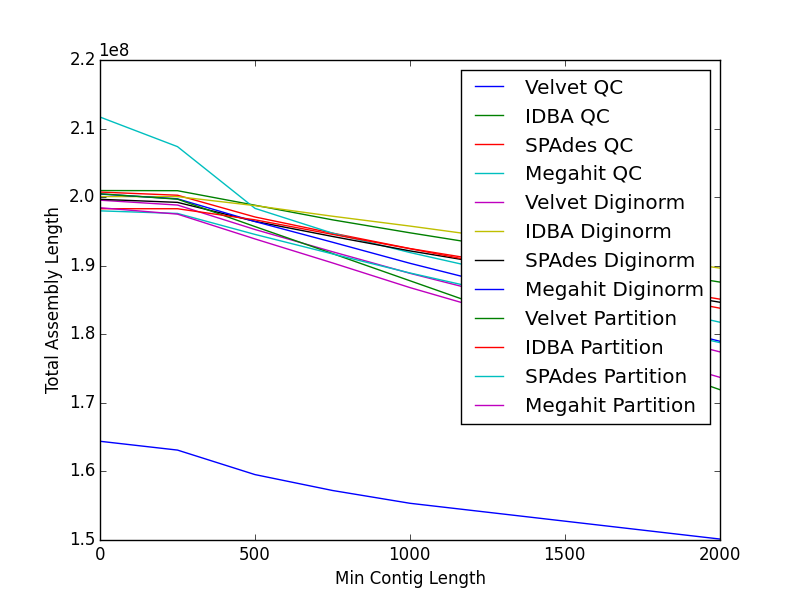
\includegraphics[height=3.2in,width=4.5in]{mincontigs.png}  
\caption{\small \sl Total Length of assemblies in basepairs based on different min contigs length.\label{fig:mincontig}}  
\end{center}  
\end{figure}  
 

\begin{figure} [h] 
\begin{center}  
 
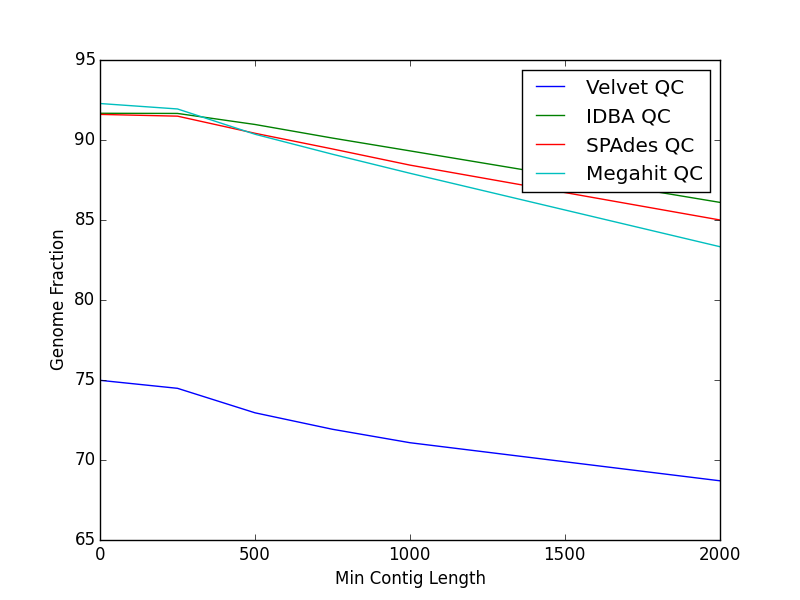
\includegraphics[height=3.2in,width=4.5in]{gfmincontig.png}  
\caption{\small \sl Genome Fraction of assemblies in basepairs based on different min contigs length.\label{fig:gf}}  
\end{center}  
\end{figure}  

\section*{Tables}
% 
% See introductory notes if you wish to include sideways tables.
%
% NOTE: Please look over our table guidelines at http://www.plosone.org/static/figureGuidelines#tables to make sure that your tables meet our requirements. Certain types of spacing, cell merging, and other formatting tricks may have unintended results and will be returned for revision.
%
%\begin{table}[!ht]
%\caption{
%\bf{Table title}}
%\begin{tabular}{|c|c|c|}
%table information
%\end{tabular}
%\begin{flushleft}Table caption
%\end{flushleft}
%\label{tab:label}
% \end{table}



%\begin{table}[t]
%\caption{Coverage Distribution}
%\centering
%\begin{tabular}{|c|c|}
%\hline
% \textbf{Covergae Range}& \textbf{No. of Reads}   \\ [0.5ex] % inserts table %heading
%\hline
%{ Between 20 and 40} & 95,540,661 \\
%\hline
%{ Between 40 and 60} &108,083 \\
%\hline
%{ Between 60 and 80} &22,677\\
%\hline
%{ Between 80 and 100} &17,148\\
%\hline
%{ Between 100 and 200} &80,878\\
%\hline
%{Coverage $\geq 200$} & 402,333\\
%\hline
%\end{tabular}
%\label{table:cov-dist} 
%\end{table}



\begin{table}[h]
\caption{Assembly Quality Metrics}
\centering
\begin{tabular}{|c|c|c|c|c|}
\hline
\textbf {Treatment/Quality Metric}& \textbf{Quality Filtering} & \textbf{Digital Normalization} & \textbf{Partition} \\ [0.5ex] % inserts table %heading
\hline
 \multicolumn{4}{|c|} {\textbf{(1) Velvet}}    \\ [0.5ex] % inserts table %heading
\hline
\textbf{Genome Fraction}& 72.949&89.043&88.879 \\
\hline
\textbf{Unaligned Length} &8,977,149&10,909,693&11,317,834\\ [1ex]
\hline
\textbf{Misassembled contigs length  }&16,566,891&25,594,315&16,922,852 \\ [1ex]
\hline
\textbf{N50} &38,028 &18,944 &8,504 \\ [1ex]
\hline
\textbf{NG50 }&22223&17212&7905  \\ [1ex]
\hline
\multicolumn{4}{|c|}{ \textbf{(2) Idba}}    \\ [0.5ex] % inserts table %heading
\hline
\textbf{Genome Fraction} &90.969&	91.003&90.082 \\   
\hline
\textbf{Unaligned Length}  &10,709,716&10,637,811&10,644,357 \\ [1ex]
\hline
\textbf{Misassembled contigs length  }&21,777,032&27,668,818&18,440,791  \\ [1ex]
\hline
\textbf{N50} &49773&47828&26575 \\ [1ex]
\hline
\textbf{NG50}&45748&44351&24326\\ [1ex]
\hline
\multicolumn{4}{|c|}{ \textbf{(3) Spades} }   \\ [0.5ex] % inserts table %heading
\hline
\textbf{Genome Fraction} &90.424&90.173&89.272\\
\hline
\textbf{Unaligned Length} &10,597,529&10,621,398&10,500,235 \\ [1ex]
\hline
\textbf{Misassembled contigs length  }&28,238,787&23,103,154&14,338,099  \\ [1ex]
\hline
\textbf{N50} &42773&35580&22319\\ [1ex]
\hline
\textbf{NG50} &38841&32598&19909\\ [1ex]
\hline
\multicolumn{4}{|c|}{ \textbf{(4) Megahit} }    \\ [0.5ex] % inserts table %heading
\hline
\textbf{Genome Fraction} &90.358&89.92&88.769 \\
\hline
\textbf{Unaligned Length}&10,686,421&10,581,435&10,564,244 \\ [1ex]
\hline
\textbf{Misassembled contigs length  }&11,927,502&17,319,534&11,814,070 \\ [1ex]
\hline
\textbf{N50} &35,136&27,302&17,492 \\ [1ex]
\hline
\textbf{NG50} &32251&25248&15393 \\ [1ex]
\hline

\end{tabular}
\label{table:qualtiy-metrics}
\end{table}


\begin{table}[h]
\caption{Running Time and Memory Utilization}
\centering
\begin{tabular}{|c|c|c|c| }
\hline
\textbf {Treatment/Quality Metric}& \textbf{Quality Filtering} & \textbf{Digital Normalization} & \textbf{Partition}  \\ [0.5ex] % inserts table %heading
\hline
 \multicolumn{4}{|c|} {\textbf{(1) Velvet}}    \\ [0.5ex] % inserts table %heading
\hline
\textbf{Running Time} &60:42:52 &6:48:46 &4:30:36   \\ 
\hline
\textbf{Memory Utilization in GB}&98.40&52.67&35.23\\ 
\hline
\multicolumn{4}{|c|}{ \textbf{(2) Idba}}    \\ [0.5ex] % inserts table %heading
\hline
\textbf{Running Time} &33:53:46&6:34:24 &8:30:29  \\ 
\hline`
\textbf{Memory Utilization in GB}&123.84&99.88&89.25\\ 
\hline
\multicolumn{4}{|c|}{ \textbf{(3) Spades} }   \\ [0.5ex] % inserts table %heading
\hline
\textbf{Running Time} &67:02:16&15:53:10&7:54:26  \\
\hline
\textbf{Memory Utilization in GB}&381.79&121.52&123.7 \\ 
\hline
\multicolumn{4}{|c|}{ \textbf{(4) Megahit} }    \\ [0.5ex] % inserts table %heading
\hline
\textbf{Running Time}&1:52:55&0:30:23&1:23:28 \\
\hline
\textbf{Memory Utilization in GB}&33.41&18.89&189.55 \\ 
\hline


\end{tabular}
\label{table:time-memory}
\end{table}



\begin{table}[h]
\caption{Misassemblies}
\centering
\begin{tabular}{|c|c|c|c|c|}
\hline
\textbf {Assembly}& \textbf{Quality Filtering} & \textbf{Digital Normalization} & \textbf{Partition} \\ [0.5ex] % inserts table %heading
\hline
 \multicolumn{4}{|c|} {\textbf{(1) Velvet}}    \\ [0.5ex] % inserts table %heading
\hline
\textbf{Misassemblies}&917&5271&5202 \\
\hline
\textbf{Relocations} &592&998&1036 \\ [1ex]
\hline
\textbf{Translocations}&309&4262&4153  \\ [1ex]
\hline
\textbf{Inversions}&16&11&13  \\ [1ex]
\hline
\textbf{Misassembled Contigs Length}&16,566,891&25,594,315&16,922,852 \\ [1ex]
\hline
\textbf{Mismatches} &104,740&174,446&178,348  \\ [1ex]
\hline 
\textbf{Percentage of Mismatches}&0.066\%&0.089\%&0.0911\%  \\[1ex]
\hline
\textbf{Indels Length}&50,190&181,453&346,988 \\ [1ex]
\hline
\textbf{Indels Percentage}&0.031\%&0.093\%&0.178\%\\ [1ex]
\hline

 \multicolumn{4}{|c|} {\textbf{(3) IDBA}}    \\ [0.5ex] % inserts table %heading
\hline
\textbf{Misassemblies}&1223&1094&960  \\
\hline
\textbf{Relocations} &613&668&578 \\ [1ex]
\hline
\textbf{Translocations}&580&398&350 \\ [1ex]
\hline
\textbf{Inversions} &30&28&32 \\ [1ex]
\hline
\textbf{Misassembled Contigs Length}&21,777,032&27,668,818&18,440,791 \\ [1ex]
\hline
\textbf{Mismatches} &162,733 &231,432&230,840 \\ [1ex]
\hline 
\textbf{Percentage of Mismatches}&0.082\%&0.116\%&0.117\% \\[1ex]
\hline
\textbf{Indels Length} &30,433&43,358&42,523  \\ [1ex]
\hline
\textbf{Indels Percentage}&0.015\%&0.022\%&0.022\%  \\ [1ex]
\hline


 \multicolumn{4}{|c|} {\textbf{(2) SPAdes}}    \\ [0.5ex] % inserts table %heading
\hline
\textbf{Misassemblies}&894&997&753 \\
\hline
\textbf{Relocations}&608&613&496 \\ [1ex]
\hline
\textbf{Translocations}&267&368&239\\ [1ex]
\hline
\textbf{Inversions}&19&16&18\\ [1ex]
\hline
\textbf{Misassembled Contigs Length}&28,238,787&23,103,154&14,338,099\\ [1ex]
\hline
\textbf{Mismatches}&184,630&244,849&235,396\\ [1ex]
\hline 
\textbf{Percentage of Mismatches}&0.093\%&0.124\%&0.120\%\\ [1ex]
\hline
\textbf{Indels Length}&27,328&32,783&21,516\\ [1ex]
\hline
\textbf{Indels Percentage}&0.014\% &0.017\%&0.011\%\\ [1ex]
\hline

 \multicolumn{4}{|c|} {\textbf{(4) Megahit}}    \\ [0.5ex] % inserts table %heading
\hline
\textbf{Misassemblies}&738&880&748 \\
\hline
\textbf{Relocations}&448&593&513\\ [1ex]
\hline
\textbf{Translocations}&172&274&222\\ [1ex]
\hline
\textbf{Inversions}&118&13&13\\ [1ex]
\hline
\textbf{Misassembled Contigs Length}&11,927,502&17,319,534&11,814,070  \\ [1ex]
\hline
\textbf{Mismatches}&152,964&207,349&203,515\\ [1ex]
\hline 
\textbf{Percentage of Mismatches}&0.078\%&0.11\%&0.10\%\\[1 ex]
\hline
\textbf{Indels Length }&15,298&18,195&16,517\\ [1ex]
\hline
\textbf{Indels Percentage}&0.008\%&0.009\%&0.008\% \\ [1ex]
\hline
\end{tabular}
\label{table:misassemblies}
\end{table}

\begin{table}[t]
\caption{Mapping quality-filtered reads to assemblies}
\centering
\begin{tabular}{|c|c|c|c|}
\hline
\textbf {Treatment}& \textbf{Quality Filtering} & \textbf{Digital Normalization} & \textbf{Partition}  \\ [0.5ex] % inserts table %heading
\hline
 \multicolumn{4}{|c|} {\textbf{(1) Velvet}}    \\ [0.5ex] % inserts table %heading
\hline
\textbf{No. of Unaligned Sequences}&6,801,329&3,375,222&3,890,205  \\ 
\hline
\textbf{Percentage}&4.26\%&1.73\%&1.99 \% \\
\hline
\multicolumn{4}{|c|}{ \textbf{(2) Idba}}    \\ [0.5ex] % inserts table %heading
\hline
\textbf{No. of Unaligned Sequences}&1,490,609&1,738,371&2,297,377 \\
\hline
\textbf{Percentage}&0.75\%&0.87\%&1.17\% \\
\hline
\multicolumn{4}{|c|}{ \textbf{(3) Spades} }   \\ [0.5ex] % inserts table %heading
\hline
\textbf{No. of Unaligned Sequences}&2,100,555&2,439,158&2,804,006\\
\hline
\textbf{Percentage}&1.06\%&1.24\%&1.44\%\\
\hline
\multicolumn{4}{|c|}{ \textbf{(4) Megahit} }    \\ [0.5ex] % inserts table %heading
\hline
\textbf{No. of Unaligned Sequences}&1,559,300&2,082,881&2,747,427 \\
\hline
\textbf{Percentage}&0.79\%&1.06\% &1.42\% \\
\hline
\end{tabular}
\label{table:reads-mapping} 
\end{table}




%\begin{table}[t]
%\caption{Mapping quality-filtered reads to assemblies}
%\centering
%\begin{tabular}{|c|c|c|c|}
%\hline
%\textbf {Treatment}& \textbf{Quality Filtering} & \textbf{Digital Normalization} & \textbf{Partition}  \\ [0.5ex] % inserts table %heading
%\hline

% \multicolumn{4}{|c|} {\textbf{(1) Velvet}}    \\ [0.5ex] % inserts table %heading
%\hline
%\textbf{No. of Unaligned Sequences}&5,553,831&521,126&667,471 \\ 
%\hline
%\textbf{Percentage}&5.22\%&0.49\%&0.63\% \\
%\hline
%\multicolumn{4}{|c|}{ \textbf{(2) Idba}}    \\ [0.5ex] % inserts table %heading
%\hline
%\textbf{No. of Unaligned Sequences} &124,846&115,323&512,264\\
%\hline
%\textbf{Percentage}&0.12\%&0.11\%&0.48\% \\
%\hline
%\multicolumn{4}{|c|}{ \textbf{(3) Spades} }   \\ [0.5ex] % inserts table %heading
%\hline
%\textbf{No. of Unaligned Sequences}&81,775&95,338&423,833 	 \\
%\hline
%\textbf{Percentage}&0.08\%&0.09\%&0.40\%\\
%\hline
%\multicolumn{4}{|c|}{ \textbf{(4) Megahit} }    \\ [0.5ex] % inserts table %heading
%\hline
%\textbf{No. of Unaligned Sequences}&80,002&88,616&468,032 \\
%\hline
%\textbf{Percentage}&0.08\%&0.08\% &0.44\% \\
%\hline
%\end{tabular}
%\label{table:reads-mapping} 
%\end{table}




\begin{table}[h]
\caption{Mapping unaligned  contigs to Idba quality-filtered  unaligned contigs }
\centering
\begin{tabular}{|c|c|c|c|c|}
\hline
\textbf {Treatment/Quality Metric}& \textbf{Quality Filtering} & \textbf{Digital Normalization} & \textbf{Partition} \\ [0.5ex] % inserts table %heading
\hline
 \multicolumn{4}{|c|} {\textbf{(1) Velvet}}    \\ [0.5ex] % inserts table %heading
\hline
\textbf{Genome Fraction}&80.613 \%&92.03\%&92.982\%   \\
\hline
\textbf{Unaligned Length}&2,475,529& 3192491&3,868,558 \\ [1ex]
\hline
\textbf{Percentage of unaligned}&37.06\%&47.8\%&57.92\%\\ [1ex]
\hline
\multicolumn{4}{|c|}{ \textbf{(2) Idba}}    \\ [0.5ex] % inserts table %heading
\hline
\textbf{Genome Fraction}&-&91.53\%&94.72\%\\   


\hline
\textbf{Unaligned Length}&-&498,299&1,320,036\\ [1ex]
\hline
\textbf{Percentage of unaligned}&-&7.46\%&19.76\% \\ [1ex]
\hline
\multicolumn{4}{|c|}{ \textbf{(3) Spades} }   \\ [0.5ex] % inserts table %heading
\hline
\textbf{Genome Fraction}&91.92\%&93.959\%&94.826\%\\
\hline
\textbf{Unaligned Length}&2,174,574&1,951,911&2,398,664\\ [1ex]
\hline
\textbf{Percentage of unaligned}&32.56\%&29.22\%&35.91\%\\ [1ex]
\hline
\multicolumn{4}{|c|}{ \textbf{(4) Megahit} }    \\ [0.5ex] % inserts table %heading
\hline
\textbf{Genome Fraction}&92.715\%&91.838\%&92.219\% \\
\hline
\textbf{Unaligned Length}&916,247&1,569,436&3,832,050 \\ [1ex]
\hline
\textbf{Percentage of unaligned}&13.72\%&23.5\%&57.37\%\\ [1ex]
\hline
\end{tabular}
\label{table:unaligned-mapping}
\end{table}


%%%%%SUPLEMENTARY TABLES 
\begin{table}[h]
\caption{Supplementary Table: More Assembly Quality Metrics}
\centering
\begin{tabular}{|c|c|c|c|c|}
\hline
\textbf {Treatment/Quality Metric}& \textbf{Quality Filtering} & \textbf{Digital Normalization} & \textbf{Partition} \\ [0.5ex] % inserts table %heading
\hline
 \multicolumn{4}{|c|} {\textbf{(1) Velvet}}    \\ [0.5ex] % inserts table %heading
\hline
\textbf{N75}&13301&6084&3771\\ [1ex]
\hline
\textbf{NG75}&1186&4805&3214\\ [1ex]
\hline
\textbf{L50} &1013&2455&6037 \\ [1ex]
\hline
\textbf{LG50} &1806&2740&6641\\ [1ex]
\hline
\textbf{L75} &2777&7026&14734\\ [1ex]
\hline
\textbf{LG75} &11087&8460&16867\\ [1ex]
\hline
\multicolumn{4}{|c|}{ \textbf{(2) Idba}}    \\ [0.5ex] % inserts table %heading
\hline
\textbf{N75}&11693&12154&7834  \\ [1ex]
\hline
\textbf{NG75} &9617	&10221&6461 \\ [1ex]
\hline
\textbf{L50}&828&896&1536\\ [1ex]
\hline
\textbf{LG50}&899&970&1712 \\ [1ex]
\hline
\textbf{L75}&2986&3025&5062 \\ [1ex]
\hline
\textbf{LG75}&3467&3484	&6002\\ [1ex]
\hline
\textbf{N75} &11263&10554&6900\\ [1ex]
\hline
\textbf{NG75} &9005	&8379&5401\\ [1ex]
\hline
\textbf{L50} &974&1192&1846\\ [1ex]
\hline
\textbf{LG50} &1078&1325&2108\\ [1ex]
\hline
\textbf{L75} &3276&3768&5840\\ [1ex]
\hline
\textbf{LG75} &3908&4495&7198\\ [1ex]
\hline
\multicolumn{4}{|c|}{ \textbf{(4) Megahit} }    \\ [0.5ex] % inserts table %heading
\hline
\textbf{N75} &8166&7230&5271 \\ [1ex]
\hline
\textbf{NG75} &6601	&5632&4030 \\ [1ex]
\hline
\textbf{L50} &1199	&1582&2490 \\ [1ex]
\hline
\textbf{LG50} &1306	&1757&2848 \\ [1ex]
\hline
\textbf{L75} &4164	&5063&7670 \\ [1ex]
\hline
\textbf{LG75} &4907&6147&9581 \\ [1ex]
\hline

\end{tabular}
\label{table:sub-qc}
\end{table}


\begin{table}[t]
\caption{Comparision between N50 and NG50}
\centering
\begin{tabular}{|c|c|c|c|}
\hline
\textbf {Treatment}& \textbf{Quality Filtering} & \textbf{Digital Normalization} & \textbf{Partition}  \\ [0.5ex] % inserts table %heading
\hline

 \multicolumn{4}{|c|} {\textbf{(1) Velvet}}    \\ [0.5ex] % inserts table %heading
\hline
\textbf{N50}&38,028&18,944&8,504 \\ 
\hline
\textbf{NG50}&22,223&17,212&7,905\\
\hline
 \multicolumn{4}{|c|} {\textbf{(2) IDBA}}    \\ [0.5ex] % inserts table %heading
\hline
\textbf{N50}&49,773&47,828&26,575 \\ 
\hline
\textbf{NG50}&45,748&44,351&24,326 \\
\hline
 \multicolumn{4}{|c|} {\textbf{(3) SPAdes}}    \\ [0.5ex] % inserts table %heading
\hline
\textbf{N50}&42,773&35,580&22,319\\ 
\hline
\textbf{NG50}&38,841&32,598&19,909\\
\hline
 \multicolumn{4}{|c|} {\textbf{(4) Megahit}}    \\ [0.5ex] % inserts table %heading
\hline
\textbf{N50}&35,136&27,302&17,492\\ 
\hline
\textbf{NG50}&32,251&25,248&15,393\\
\hline
\end{tabular}
\label{table:n50-ng50} 
\end{table}





\section *{Supporting Information Legends} 
%
% Please enter your Supporting Information captions below in the following format:
%\item{\bf Figure SX. Enter mandatory title here.} Enter optional descriptive information here.
% 
%\begin{description}
%\item {\bf}
%\item {\bf}
%\end{description}

\end{document}

